---
title: Higher Homotopy Groupoids
numbersections: true
---

\section{Preliminaries: Categories}

\subsection{Basics}

\begin{dfn}[Category]
	A \emph{category} $\cC$ consists of a collection of \emph{objects} $\Obj(\cC)$
	and a collection of \emph{morphisms} $\Hom(\cC)$, such that

	\begin{itemize}
		\item Each morphism $f$ has a specific \emph{domain} $\dom(f)$ and
		      \emph{codomain} $\cod(f)$; we write $f: X\rightarrow Y$ or
		      $X\xrightarrow{f} Y$.
		\item Each object $X$ has a specific \emph{identity morphism} $1_X:
			      X\rightarrow X$.
		\item For each pair of morphisms $X\xrightarrow{f} Y\xrightarrow{g}
			      Z$, there is a specific \emph{composite morphism} $gf:
			      X\rightarrow Z$.
	\end{itemize}
	This data must be \emph{associative} and \emph{unital}, which is to say,
	\begin{itemize}
		\item (Associativity) For any triplet of composition-compatible morphisms
		      $X\xrightarrow{f}Y \xrightarrow{g}Z\xrightarrow{h}W$, we have $h(gf) =
			      (hg)f$. We write merely $hgf$.
		\item (Unital) For any $f: X\rightarrow Y$, we have $1_Yf = f = f1_X$.
	\end{itemize}

	In other words, the following diagrams commute:

	\begin{figure}[H]
		\centering
		\begin{multicols}{2}
			\begin{tikzcd}
				X & Y & Z & W
				\arrow["f", from=1-1, to=1-2]
				\arrow["g", from=1-2, to=1-3]
				\arrow["h", from=1-3, to=1-4]
				\arrow["gf"', curve={height=18pt}, from=1-1, to=1-3]
				\arrow["hg", curve={height=-18pt}, from=1-2, to=1-4]
			\end{tikzcd}

			\begin{tikzcd}
				X & X \\
				& Y
				\arrow["1_X", from=1-1, to=1-2]
				\arrow["f", from=1-2, to=2-2]
				\arrow["f"', from=1-1, to=2-2]
			\end{tikzcd}
			\begin{tikzcd}
				X & Y \\
				& Y
				\arrow["f", from=1-1, to=1-2]
				\arrow["1_Y", from=1-2, to=2-2]
				\arrow["f"', from=1-1, to=2-2]
			\end{tikzcd}
		\end{multicols}
	\end{figure}
\end{dfn}

\begin{notation}
	I will use $\cC(X, Y)$ for the collection of morphisms with domain $X$ and
	codomain $Y$. I also choose to use multiplicative notation for composition,
	instead of $\circ$, to distinguish it from composition of continuous
	functions, since in many of our categories morphism composition will be
	concatenation, not function composition.
\end{notation}

There are numerous special kinds of morphisms. We define some now.

\begin{dfn}[Isomorphism]
	A morphism $f: X\rightarrow Y$ is an \emph{isomorphism} if there is a morphism
	$g: Y\rightarrow X$ such that $gf = 1_X$ and $fg = 1_Y$. We say $X$ and $Y$
	are isomorphic and write $X\cong Y$.
\end{dfn}

\begin{thm}\label{functors preserve isomorphism}
	Let $F: \cC\rightarrow \cD$ be a functor and $f: X\rightarrow Y$ an isomorphism in
	$\cD$. Then $F(f)$ is an isomorphism between $F(X)$ and $F(y)$ in $\cD$.
\end{thm}

\begin{proof}
	Let $f^{-1}$ be the inverse of $f$. Then $$F(f^{-1})F(f) = F(f^{-1}f) = F(1_x)
		= 1_{F(x)},$$ and the same works on the other side.
\end{proof}


\subsection{Groups and Groupoids}

% TODO



\section{The Fundamental Groupoid}
\label{The Fundamental Group}

\begin{notation}
	When the context is unclear, we will call a general homotopy a \emph{free
		homotopy}, and a homotopy with fixed endpoints a \emph{path homotopy}.
\end{notation}

Before defining the fundamental groupoid, there is a nice geometric picture to
tell about the fundamental group. Fix a topological space $X$ and a point $x_0$.
Draw a representative of each of the non-identity homotopy classes of loops at
$x_0$, and note that each arrow is double-sided, since paths can be traversed in
either direction. When you "erase" the other information of the underlying
space, you get a single point and a bunch of double-headed arrows: exactly the
"categories-as-dots-and-arrows" picture of a group!

\begin{figure}[H]
	\centering
	\usetikzlibrary{decorations.markings}

\newcommand{\pathA}{(2, 2) .. controls (3,2) and (3, 1.5) .. (4, 1.5)}
\newcommand{\pathB}{(4, 1.5) .. controls (5, 1.5) and (5,2) .. (6, 2)}
\newcommand{\pathC}{(6, -2) .. controls (5,-2) and (5, -1.5) .. (4, -1.5)}
\newcommand{\pathD}{(4, -1.5) .. controls (3, -1.5) and (3,-2) .. (2, -2)}

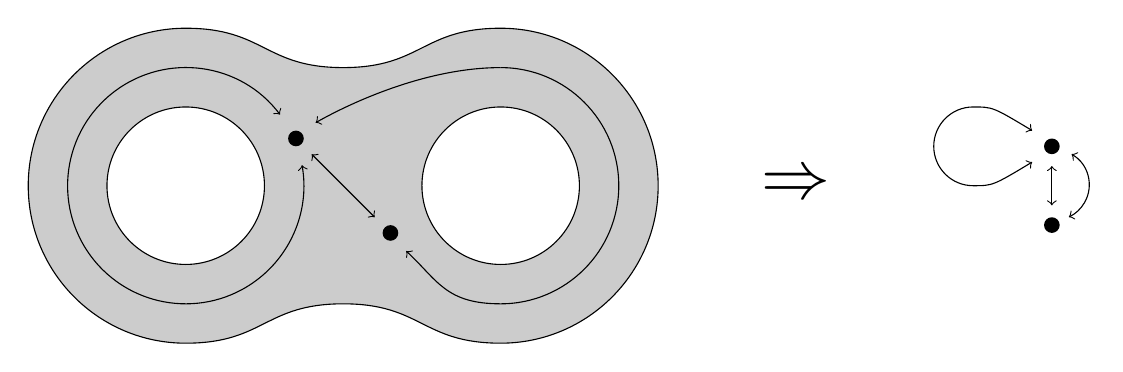
\begin{tikzpicture}
	% outer shape
	\filldraw[fill=black, fill opacity=0.2, draw=black] (0, 0) arc(180:90:2) --
	\pathA --
	\pathB --
	(6, 2) arc(90:0:2) --
	(8, 0) arc(360:270:2) --
	\pathC --
	\pathD --
	(2, -2) arc(270:180:2)
	;

	% inner holes
	\filldraw [fill=white] (2,0) circle (1);
	\filldraw [fill=white] (6,0) circle (1);

	% paths
	\coordinate (x) at (3.4, 0.6);
	\coordinate (y) at (4.6, -0.6);
	\node [circle, fill, inner sep=2pt] at (x) {};
	\draw[<->] ([shift=(37:1.5)]2,0) arc(37:370:1.5);
	\draw[<-] (3.65, 0.8) .. controls (4,1) and (5,1.5) .. (6, 1.5);
	\draw[<-] (4.8, -0.83) .. controls (5.2,-1.2) and (5.3, -1.5) .. (6, -1.5);
	\draw ([shift=(270:1.5)]6,0) arc(270:450:1.5);

	\node [circle, fill, inner sep=2pt] at (y) {};
	\draw[<->] (3.6, 0.4) -- (4.4, -0.4);

	\node[font={\Huge\Huge\bfseries\sffamily}] at (9.75, 0) {$\Rightarrow$};

	% the group!
	\coordinate (x) at (13, 0.5);
	\coordinate (y) at (13, -0.5);
	\node [circle, fill, inner sep=2pt] at (x) {};
	\node [circle, fill, inner sep=2pt] at (y) {};
	\draw[<->] (12.75, 0.7) .. controls (12.25,1.0) .. (12,1.0) --
	(12,1.0) arc(90:270:0.5) --
	(12,0) .. controls (12.25,0) .. (12.75, 0.3)
	;
	\draw[<->] (13.25, 0.4) arc (60:-65:0.45);
	\draw[<->] (13, 0.25) -- (13, -0.25);
\end{tikzpicture}

	\caption{Generators of the fundamental group on a two-holed disk.}
	\label{fig:group}
\end{figure}

We'll keep returning to this intuition of homotopy groups "erasing" some of the
underlying geometry of the space. More immediately, however, this view strongly
suggests that when we take multiple points from our underlying space, we should
get back a group with multiple objects---a groupoid---from the construction.

\begin{dfn}[Fundamental Groupoid]
	The \textit{fundamental groupoid} $\Pi_1(X)$ of a space $X$ is the category
	whose objects are points of $X$ and whose morphisms are path homotopy classes
	of paths in $X$.
\end{dfn}

Specifically, let $x,y,z\in X$, $f$ a path from $x$ to $y$, and $g$ a path from
$y$ to $z$. Then,

\begin{itemize}
	\item A path's domain is its startpoint: $\dom([f]) = x$.
	\item A path's codomain is its endpoint: $\cod([f]) = y$.
	\item The identity is the constant map: $1_x = [c_x]$.
	\item Composition is concatenation: $[g][f] = [f*g]$.
\end{itemize}

This construction is well-defined specifically because we are working with path
homotopies. For example, in general two paths with different start points may be
free homotopic, meaning without restricting to path homotopy we could not even
write down the domain and codomain of our morphisms.

\begin{ex}
	We can immediately compute a few fundamental groupoids. [Brown p. 213]
	\begin{itemize}
		\item The fundamental groupoid of a convex space is a \emph{tree groupoid},
		      i.e. a groupoid with precisely one morphism between any two objects. This
		      corresponds to the fact that any two paths with the same endpoints in such
		      a space are homotopic via the straight line homotopy.
		\item The fundamental groupoid of a totally disconnected space is a
		      \emph{discrete groupoid}, i.e. a groupoid with only identity morphisms.
		      This corresponds to the fact that the only paths in such spaces are the
		      constant paths.
	\end{itemize}
\end{ex}

\begin{prop}\label{fundamental groupoid is a groupoid}
	The fundamental groupoid is a groupoid.
\end{prop}

\begin{proof}
	All of this work was already done in class for the fundamental group. We
	restate the results here for groupoids.
	\begin{itemize}
		\item Composition is well-defined, since concatenation preserves homotopy
		      equivalence.
		\item Composition is associative, since concatenation is associative up to
		      homotopy.
		\item Every object $x$ has $[c_x]$ as an identity.
		\item Every morphism $[f]$ has $[\bar{f}]$ as an inverse.
	\end{itemize}

	The first three say that $\Pi_1(X)$ is a category, and the last says that it
	is a groupoid.
\end{proof}

The construction of the fundamental groupoid naturally gives rise to a functor
$$\Pi_1: \catname{Top}\rightarrow\catname{Grpd}.$$ In particular, let $f: X\rightarrow
	Y$ be a continuous function. We can view $f$ as acting on paths via composition.
Accordingly, we define
\begin{align*}
	\Pi_1(f)  \colon \Pi_1(X) & \to \Pi_1(Y)            \\
	[\gamma]                  & \mapsto [f\circ\gamma].
\end{align*}

% TODO: picture

This mapping is well-defined because composition preserves homotopy equivalence.

% TODO: output is a homomorphism

\begin{prop}\label{fundamental groupoid is a functor}
	$\Pi_1$ is a functor.
\end{prop}

\begin{proof}
	Again, much of this work was done in class.
	\begin{itemize}
		\item $\Pi_1$ respects composition, since composition is associative.
		\item $\Pi_1$ respects the identity, since composition by the identity
		      fixes homotopy classes. \qedhere
	\end{itemize}
\end{proof}

This result is an improvement over the fundamental group, where we needed a
functor out of based spaces for the definition to make sense. This is a first
hint that the fundamental groupoid in some sense captures more of the structure
of a space than the fundamental group does.

\begin{cor}\label{fundamental groupoid is topological}
	The fundamental groupoid is a topological invariant. More precisely, if
	$X\cong Y$, then $\Pi_1(X)\cong \Pi_1(Y)$.
\end{cor}

\begin{proof}
	This follows from \Cref{functors preserve isomorphism} and \Cref{fundamental
		groupoid is a functor}.
\end{proof}

\begin{thm}\label{fundamental groupoid is homotopy invariant}
	The fundamental groupoid is a homotopy invariant. More precisely, if $X\simeq
		Y$, then $\Pi_1(X)\cong \Pi_1(Y)$.
\end{thm}

This theorem is harder than topological invariance, because it tells us
something specific about the functor $\Pi_1$.

% TODO: what does the correct result look like? e.g. Dn and 1 have different
% groupoids (because of cardinality), but maybe the same up to some kind of
% natural isomorphism of categories

\begin{proof}

\end{proof}
